% Generated by scripts/analyze_results.py from results.csv.
% Do not edit by hand: regenerate with the command in assets/plots/README.md.

% Requires \usepackage{graphicx}.
% Paths assume the report is compiled from assets/report/.

\begin{figure}[htbp]
  \centering
  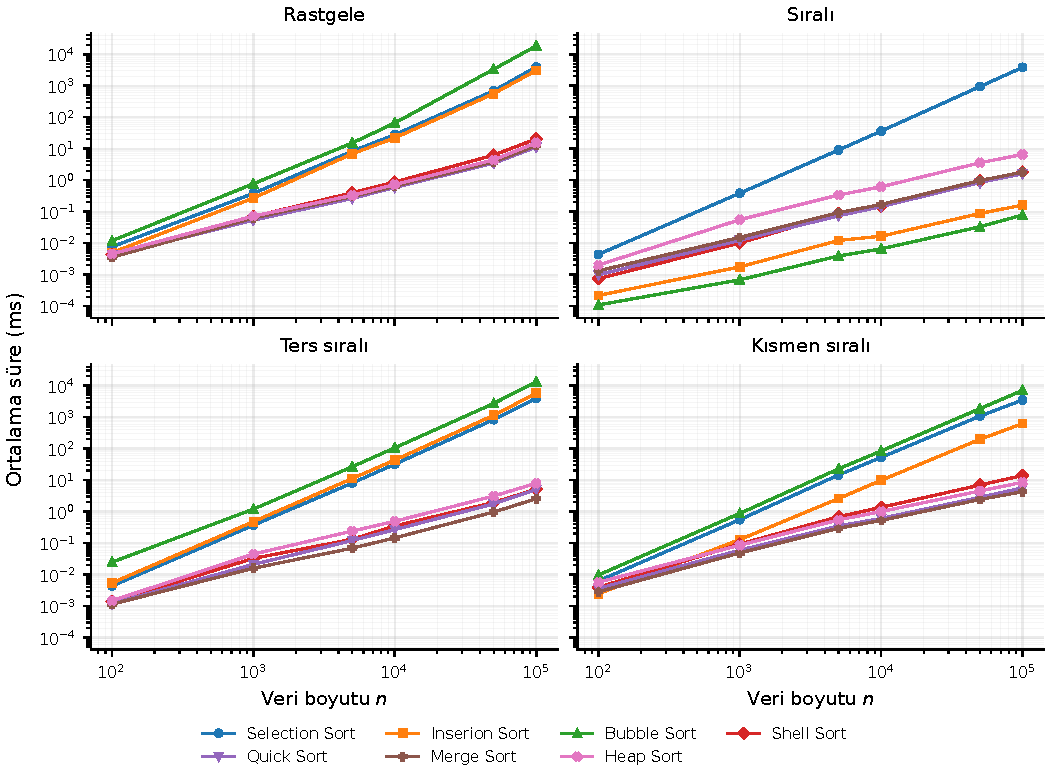
\includegraphics[width=\linewidth]{../plots/figures/fig_time_vs_n.pdf}
  \caption{Dört veri dağılımı için ortalama çalışma süresinin veri
           boyutuna göre değişimi (log--log eksenler, 5 yineleme
           ortalaması).}
  \label{fig:time}
\end{figure}

\begin{figure}[htbp]
  \centering
  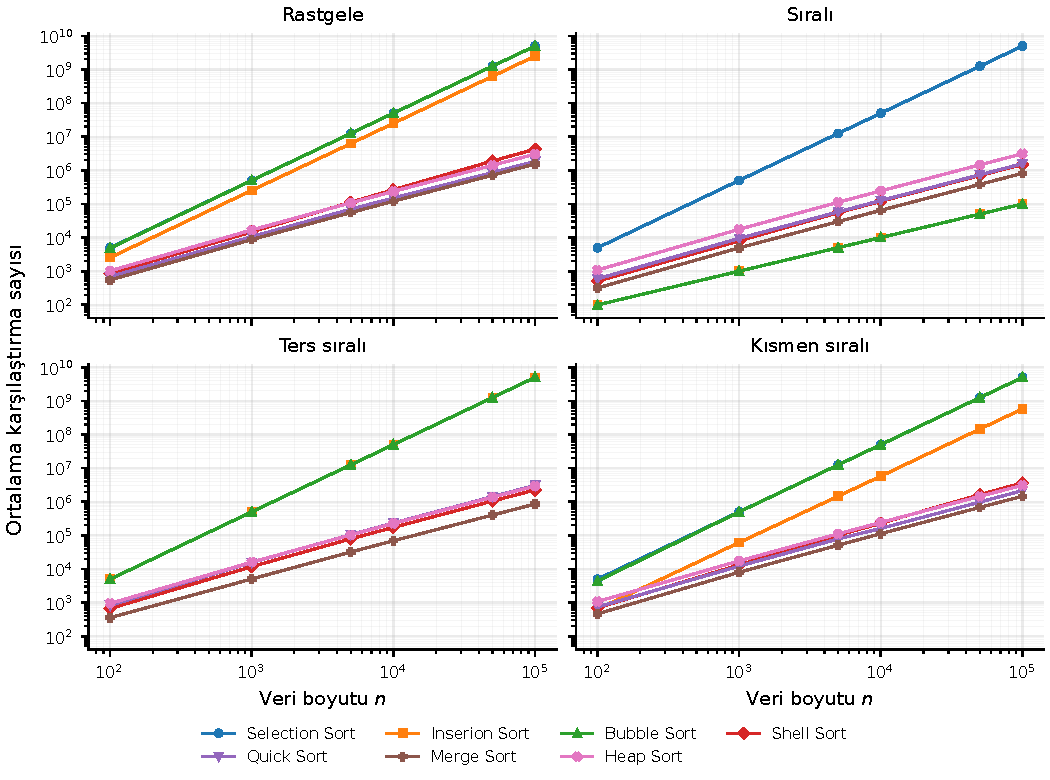
\includegraphics[width=\linewidth]{../plots/figures/fig_comparisons_vs_n.pdf}
  \caption{Ortalama karşılaştırma sayısının veri boyutuna göre değişimi
           (log--log eksenler, 5 yineleme ortalaması).}
  \label{fig:comparisons}
\end{figure}

\begin{figure}[htbp]
  \centering
  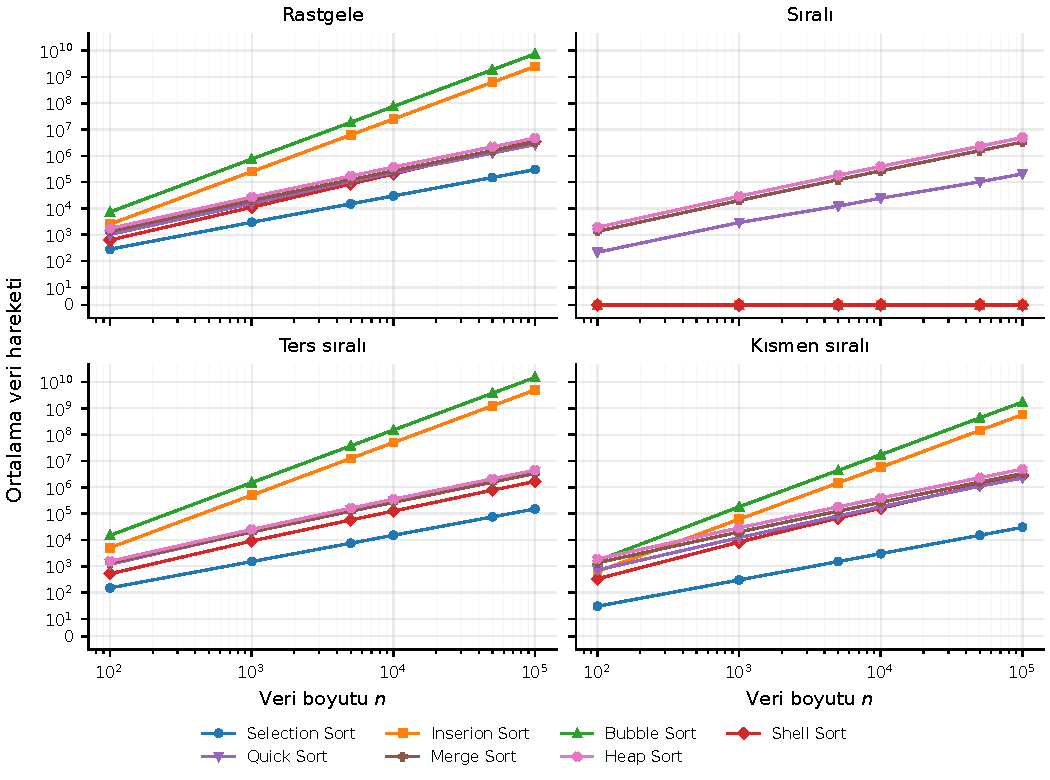
\includegraphics[width=\linewidth]{../plots/figures/fig_moves_vs_n.pdf}
  \caption{Ortalama veri hareketi sayısının veri boyutuna göre değişimi
           (5 yineleme ortalaması). Bir yer değiştirme üç hareket
           sayılmıştır; sıfır hareketli durumların görünmesi için düşey eksen
           simetrik logaritmik ölçektedir.}
  \label{fig:moves}
\end{figure}

\begin{figure}[htbp]
  \centering
  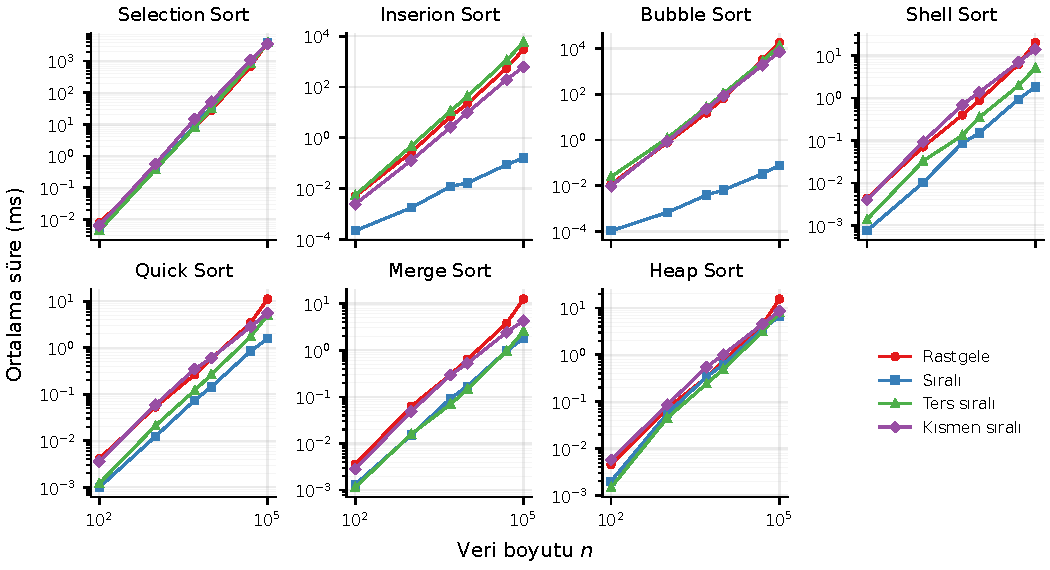
\includegraphics[width=\linewidth]{../plots/figures/fig_distribution_effect.pdf}
  \caption{Veri dağılımının çalışma süresine etkisi; her panel bir algoritma
           (log--log eksenler, 5 yineleme ortalaması).}
  \label{fig:distribution}
\end{figure}
